\section{实验结果}

\subsection{光谱仪的标定}

\subsubsection{可见光谱仪的标定}

用氘灯对可见光谱仪进行标定;调整积分时间为 10 \si{ms},打开氘灯,在空白条件下扫描得到氘灯的发射谱图如图 \ref{fig:1} 所示。

\begin{figure}[H]
    \centering
    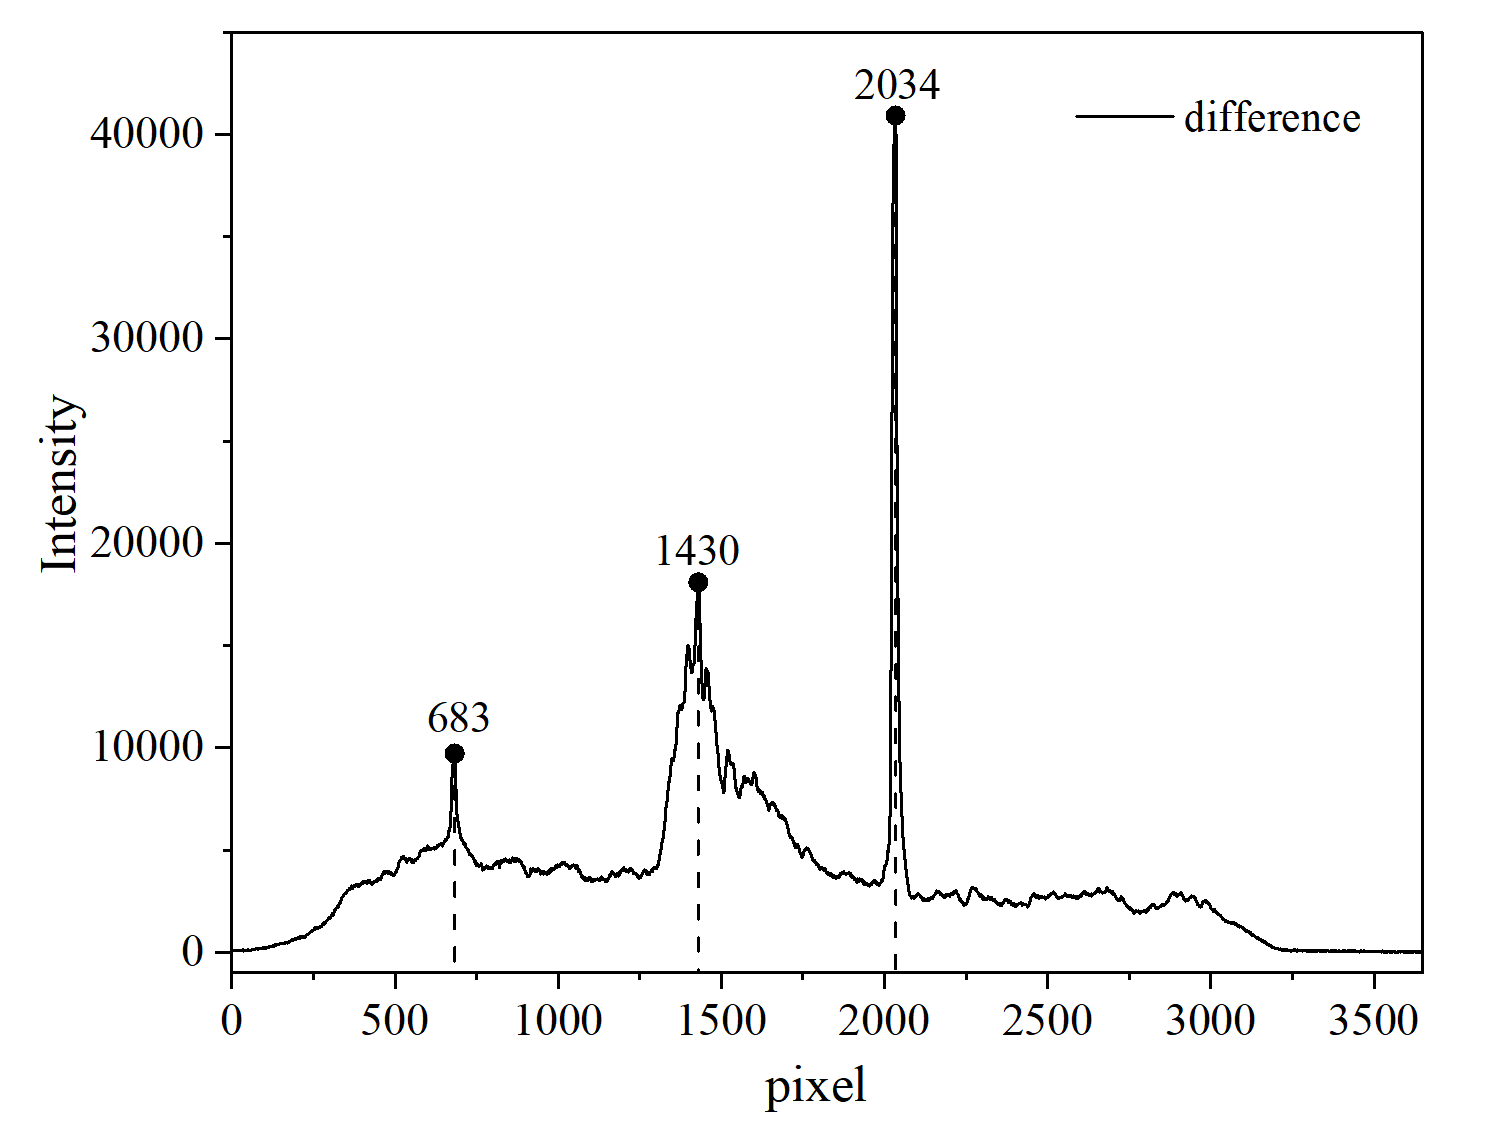
\includegraphics[width=.6\textwidth]{figures2/1-1.png}
    \bicaption{氘灯的光强-像素图:可见}{Deuterium Lamp Intensity-Pixel Map: Visible}
    \label{fig:1}
\end{figure}

取其中三个特征峰,将其与标准谱图的特征峰位置进行对比,得到表 \ref{tab:1},对三组数据进行线性拟合得到图 \ref{fig:2},线性拟合的关系式为:

\begin{equation}\label{eq:1}
    \lambda_{\rm max} = (0.12609 \pm 0.00123)\times\mathrm{pixel}+(400.13141 \pm 1.82574);\quad R^2=0.99981
\end{equation}

\begin{table}[H]
    \centering
    \bicaption{特征像素点与标准谱对应的波长:可见}{Characteristic Pixel Points and Corresponding Wavelengths of Standard Spectrum: Visible}
    \begin{tabular}{ccc}
    \toprule
    编号 & 像素值 & 波长/ \si{nm}\\
    \midrule
    1 & 683 & 485.82 \\
    2 & 1430 & 581.39 \\
    3 & 2034 & 656.06 \\
    \bottomrule
    \end{tabular}
    \label{tab:1}
\end{table}

\begin{figure}[H]
    \centering
    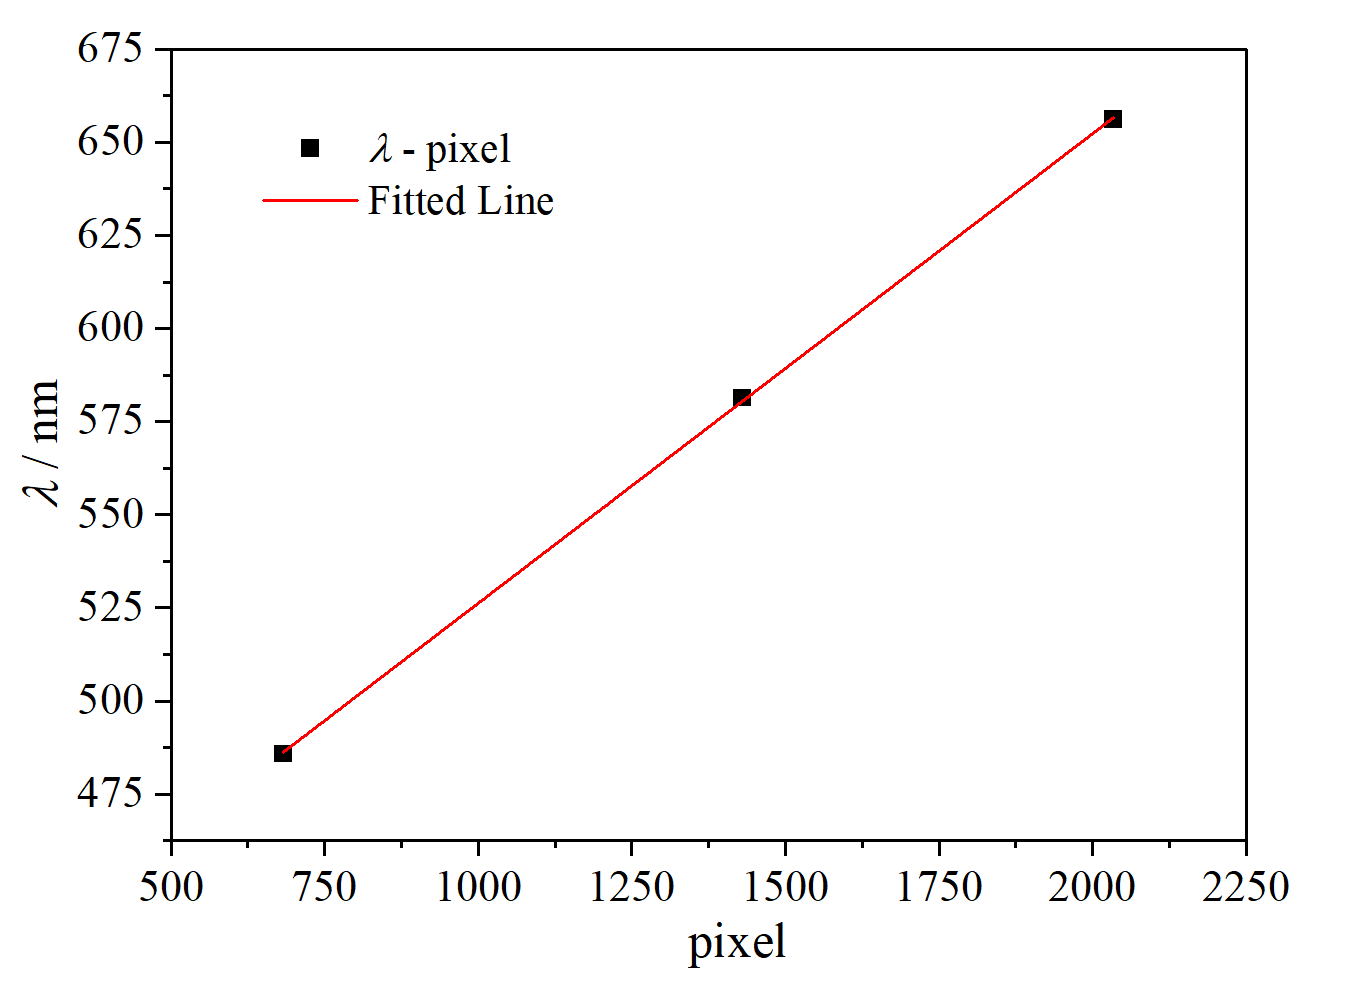
\includegraphics[width=.6\textwidth]{figures2/1-2.png}
    \bicaption{氘灯标定的标准波长-像素拟合直线:可见}{Standard Wavelength-Pixel Calibration Line for Deuterium Lamp: Visible}
    \label{fig:2}
\end{figure}

本实验中,所用的CCD像素点范围为$1\thicksim 3648$,由回归直线表达式 \eqref{eq:1} 可得可测量的光谱范围为 $400.1\thicksim 860.2 \si{nm}$,能够用于测定A组分子的吸收光谱。

\subsubsection{紫外-可见光谱仪的标定}

用氘灯对可见光谱仪进行标定;调整积分时间为 4 \si{ms},打开氘灯,在空白条件下扫描得到氘灯的发射谱图如图 \ref{fig:3} 所示。

\begin{figure}[H]
    \centering
    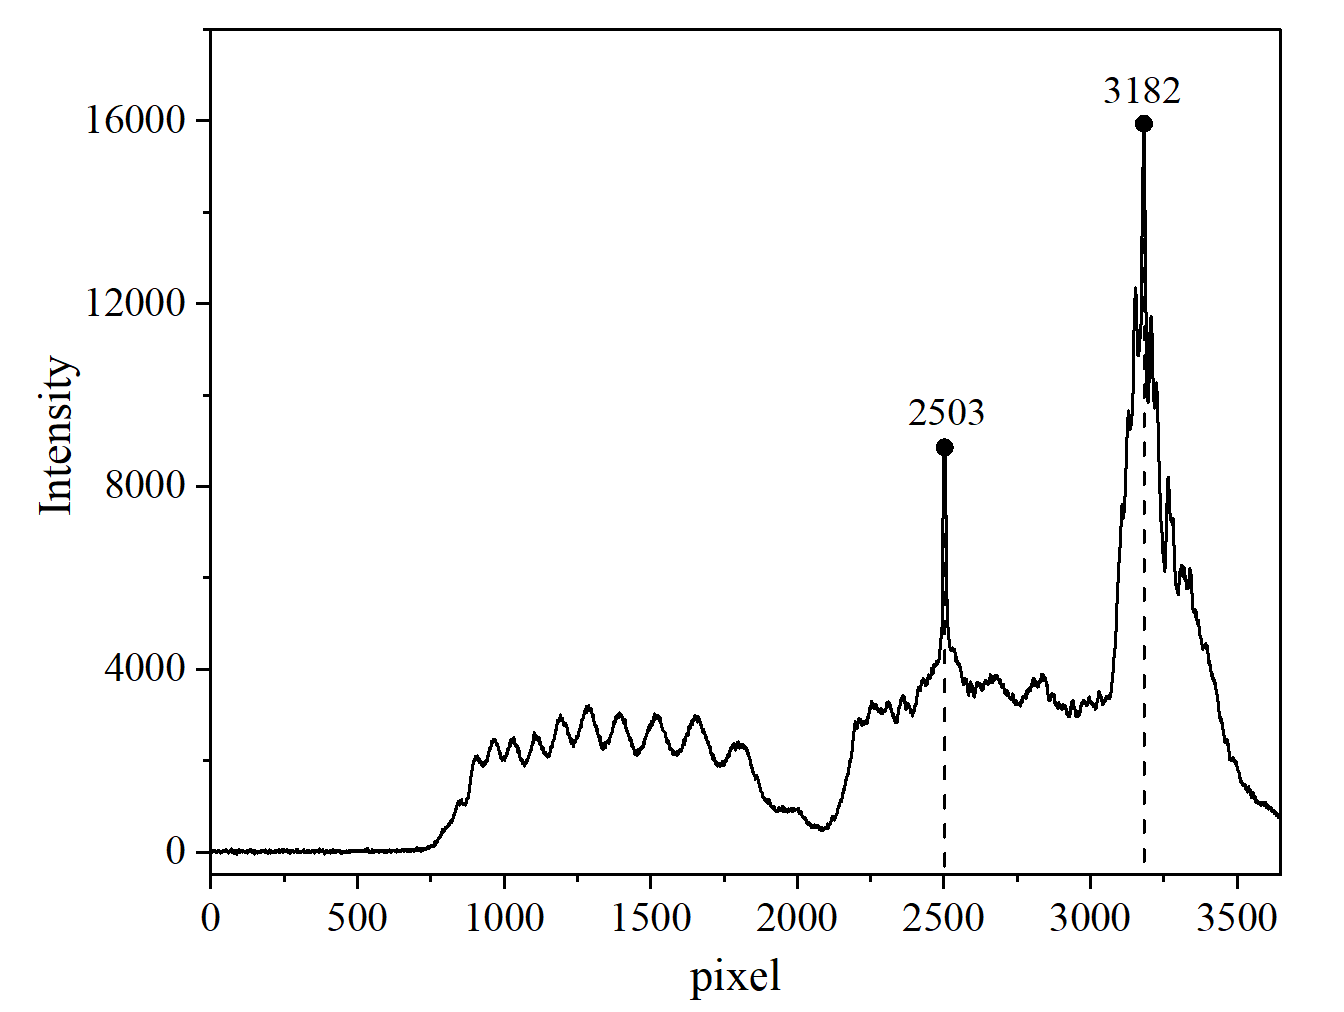
\includegraphics[width=.6\textwidth]{figures2/1-3.png}
    \bicaption{氘灯的光强-像素图:紫外-可见}{Deuterium Lamp Intensity-Pixel Map: UV-vis}
    \label{fig:3}
\end{figure}

取其中三个特征峰,将其与标准谱图的特征峰位置进行对比,得到表 \ref{tab:2},对两组数据进行线性方程求解得到图 \ref{fig:4},线性关系式为:

\begin{equation}\label{eq:2}
    \lambda_{\rm max} = 0.14054 \times \mathrm{pixel}+ 133.19481
\end{equation}

\begin{figure}[H]
    \centering
    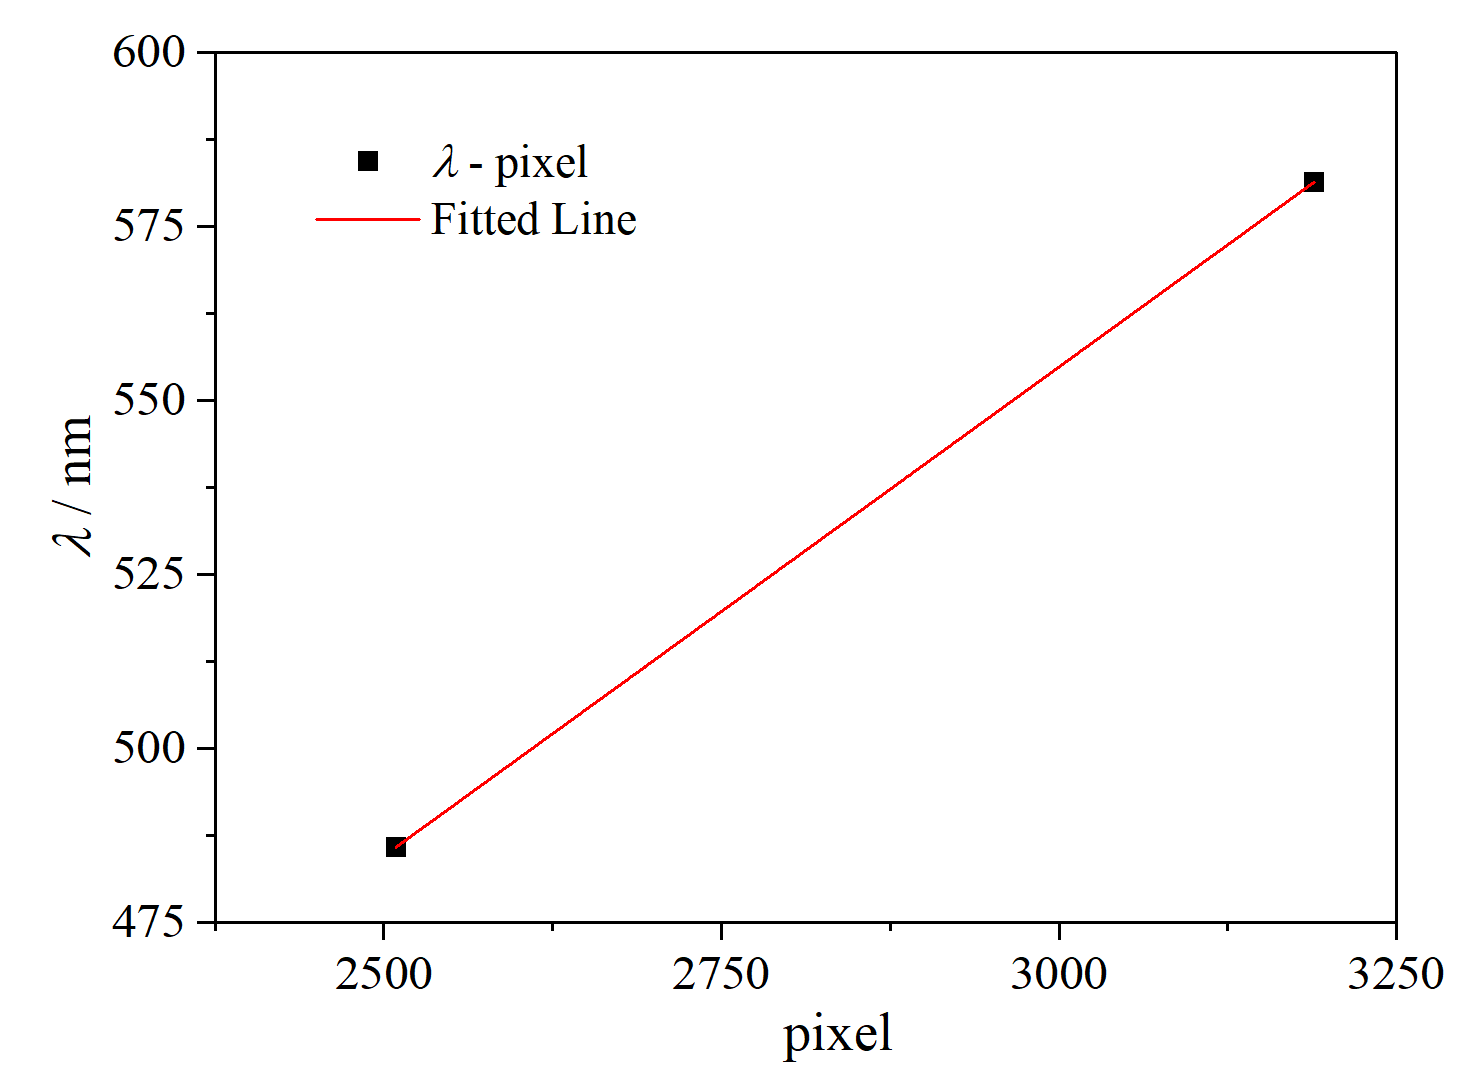
\includegraphics[width=.6\textwidth]{figures2/1-4.png}
    \bicaption{氘灯标定的标准波长-像素的线性关系:紫外-可见}{Linear Relationship of Standard Wavelength-Pixel Calibration for Deuterium Lamp: UV-vis}
    \label{fig:4}
\end{figure}

\begin{table}[H]
    \centering
    \bicaption{特征像素点与标准谱对应的波长:紫外-可见}{Characteristic Pixel Points and Corresponding Wavelengths of Standard Spectrum: UV-vis}
    \begin{tabular}{ccc}
    \toprule
    编号 & 像素值 & 波长/ \si{nm}\\
    \midrule
    1 & 2509 & 485.82 \\
    2 & 3189 & 581.39 \\
    \bottomrule
    \end{tabular}
    \label{tab:2}
\end{table}

本实验中,所用的CCD像素点范围为$1\thicksim 3648$,由直线表达式 \eqref{eq:1} 可得可测量的光谱范围为 $400.1\thicksim 860.2 \si{nm}$,能够用于测定A1以及B组分子的吸收光谱。

\subsection{测定样品的最大吸收波长与吸光度}

\subsubsection{不同浓度A3的乙醇溶液的吸收光谱测定}

使用可见光谱仪,根据线性关系 \eqref{eq:1} 将像素坐标变换为波长,扣除暗背景,利用公式计算吸光度:
\begin{equation*}
    A = \ln{\frac{I_0}{I}}
\end{equation*}
其中,$I_0$为空白溶剂乙醇的透射光强,$I$为样品的透射光强,最终得到不同浓度A3的乙醇溶液的吸收光谱,如图 \ref{fig:5}。

\begin{figure}[H]
    \centering
    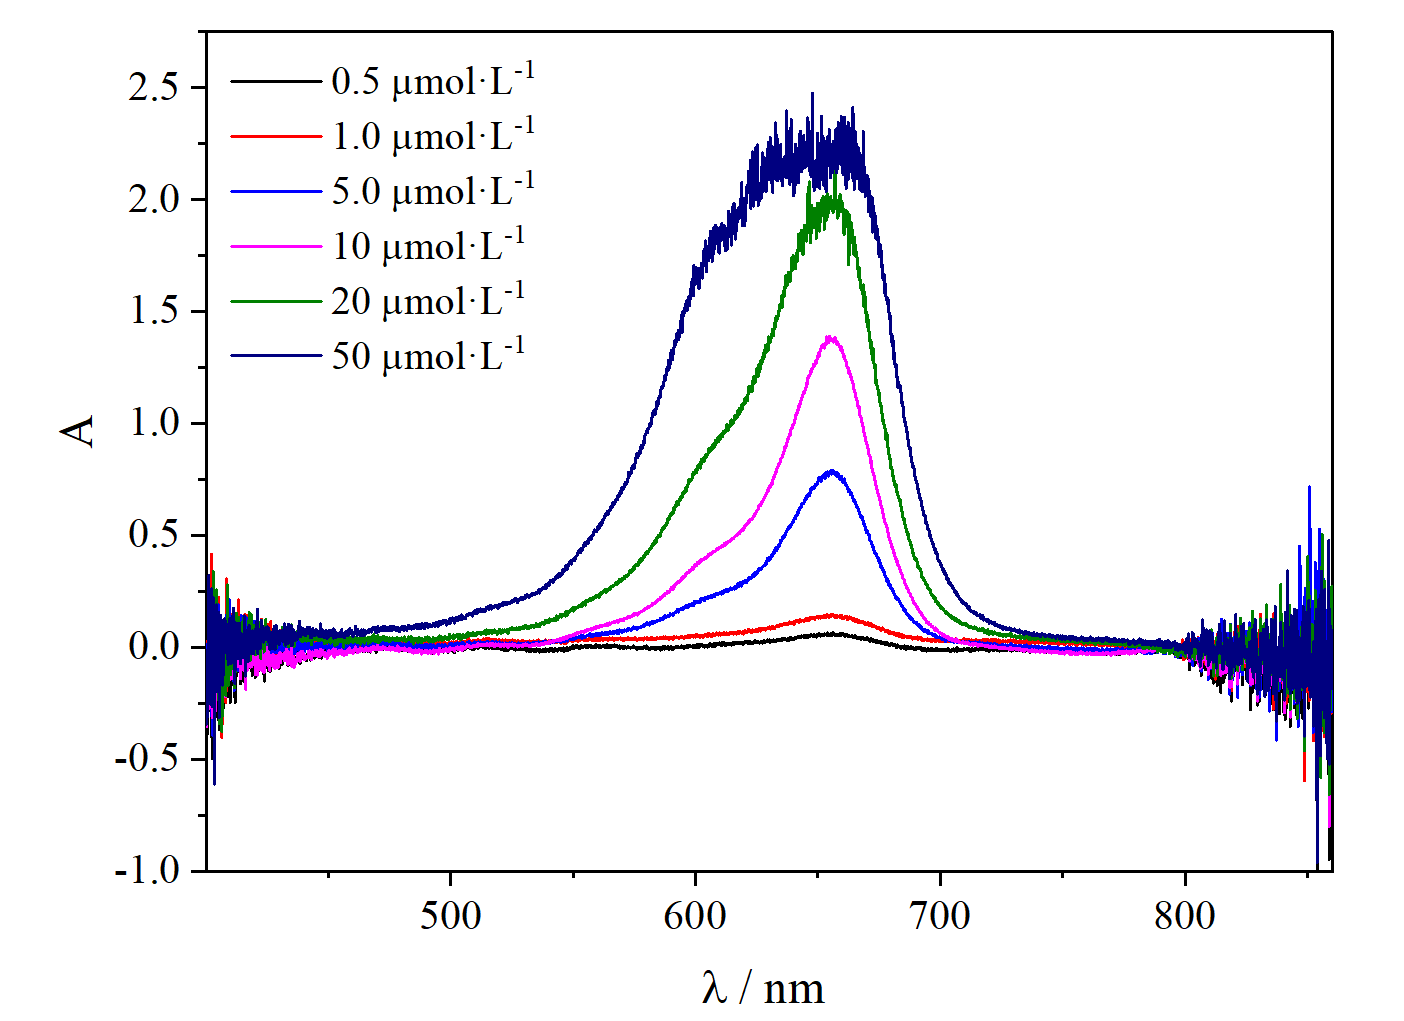
\includegraphics[width=.6\textwidth]{figures2/2-1.png}
    \bicaption{不同浓度A3的乙醇溶液的吸收光谱}{Absorption Spectrum of Ethanol Solutions of Different Concentrations A3}
    \label{fig:5}
\end{figure}

将图 \ref{fig:5} 中的曲线平滑化处理,得到图 \ref{fig:6}。

\begin{figure}[H]
    \centering
    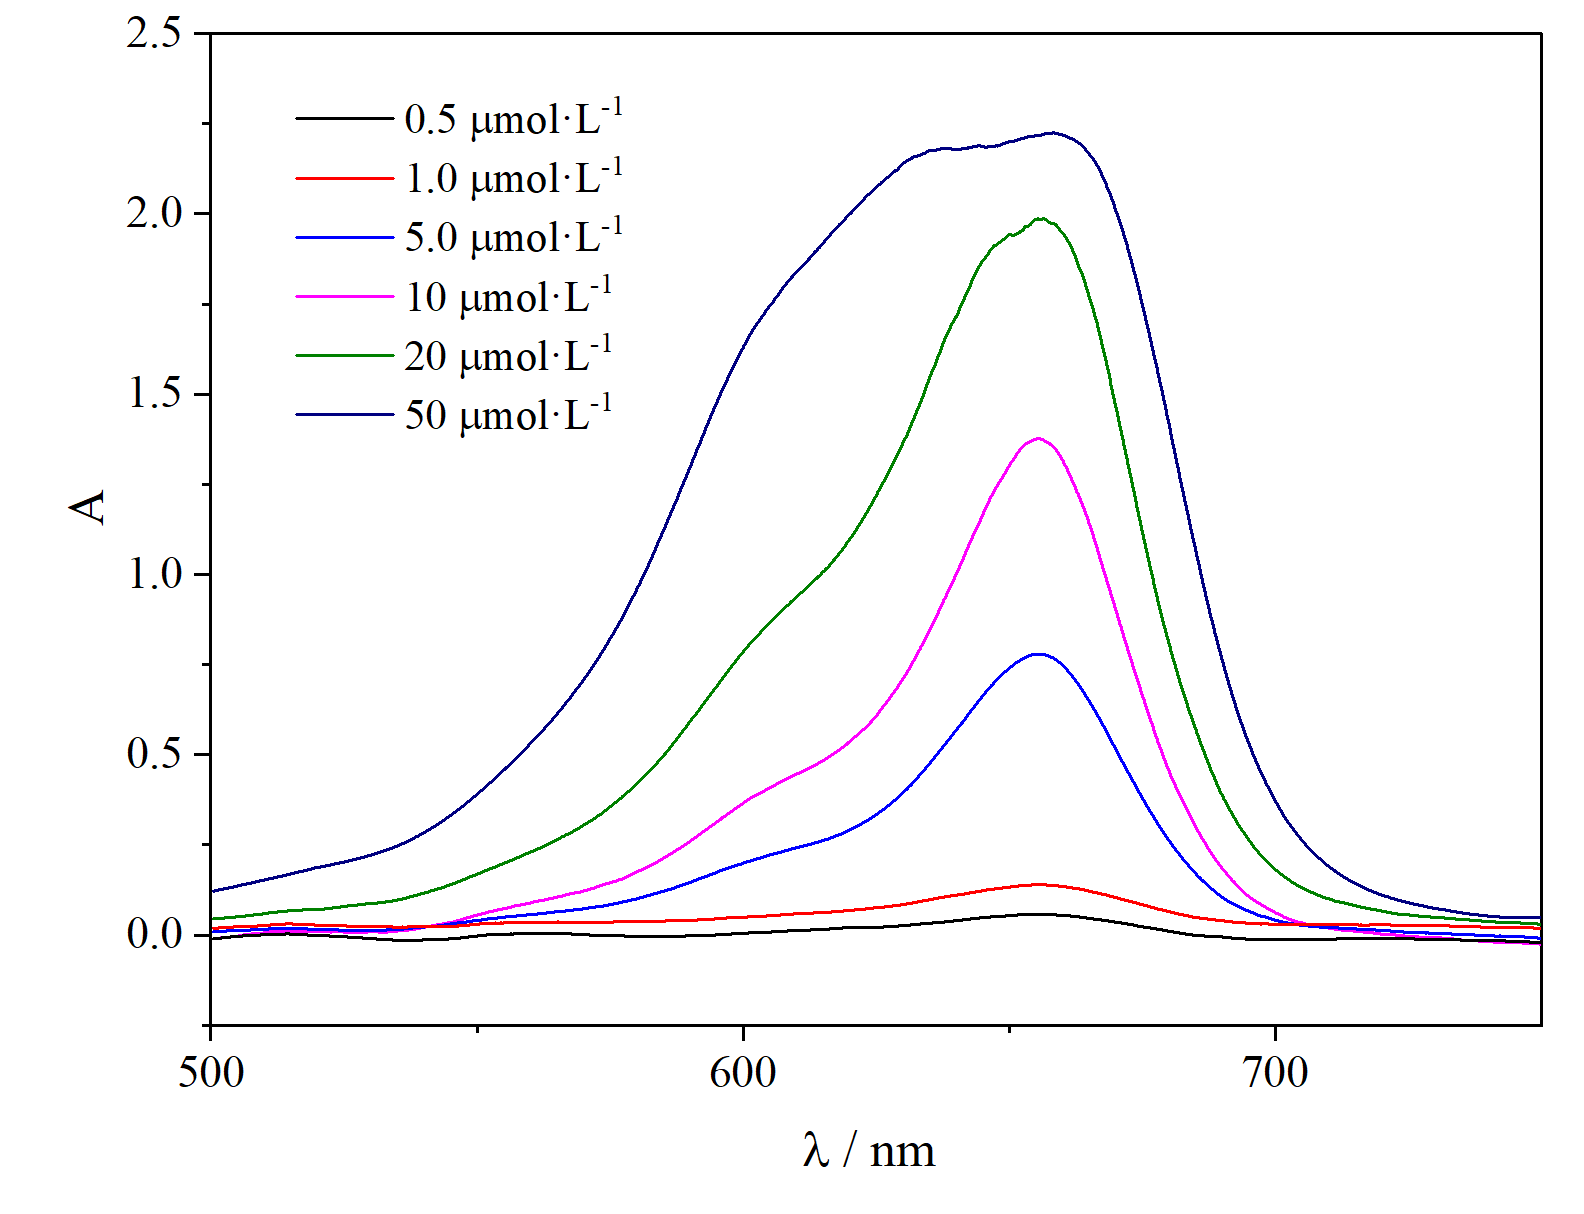
\includegraphics[width=.6\textwidth]{figures2/2-4.png}
    \bicaption{平滑化后不同浓度A3的乙醇溶液的吸收光谱}{Smoothed Absorption Spectrum of Ethanol Solutions of Different Concentrations A3}
    \label{fig:6}
\end{figure}

在图 \ref{fig:6} 中,确定不同浓度A3的乙醇溶液的最大吸收光波长与吸光度,得到表 \eqref{tab:3},做吸光度-浓度图,得到图 \ref{fig:7}。

\begin{table}[H]
    \centering
    \bicaption{不同浓度A3的乙醇溶液的吸收光波长与吸光度}{Absorption Wavelength and Absorbance of Ethanol Solutions of Various Concentrations A3}
    \begin{tabular}{cccc}
    \toprule
         编号 & 浓度/$\mathrm{\mu mol\cdot L^{-1}}$ & 吸收光波长/$\mathrm{nm}$ & 吸光度 \\
         \midrule
         1 & 0.5 & 657.1 & 0.0565 \\
         2 & 1.0 & 656.3 & 0.1388 \\
         3 & 5.0 & 655.6 & 0.7790 \\
         4 & 10 & 655.5 & 1.377 \\
         5 & 20 & 656.5 & 1.988 \\
         6 & 50 & 658.4 & 2.225 \\
         \bottomrule
    \end{tabular}
    \label{tab:3}
\end{table}
\begin{equation}\label{eq:3}
    A = \varepsilon c b
\end{equation}
根据图 \ref{fig:7} 可以发现,溶液浓度为 \SI{20}{\mu mol\cdot L^{-1}}与 \SI{50}{\mu mol\cdot L^{-1}}与低浓度时的吸光度相比,偏离了Lambert-Beer定律 \eqref{eq:3} 所揭示的的线性关系,这主要有以下两方面原因:
\begin{enumerate}
    \item Lambert-Beer定律的吸光度-浓度线性关系仅在低浓度的稀溶液中适用,而在高浓度时,会自发地偏离线性。
    \item 卤钨灯的光强有限,在高浓度时,几乎所有的透射光均被溶液所吸收,在图 \ref{fig:5} 中,可以发现 \SI{50}{\mu mol\cdot L^{-1}}时的峰顶部出现了很强的噪声,这正是由于透光率太低导致信噪比升高所导致的。
\end{enumerate}

\begin{figure}[H]
    \centering
    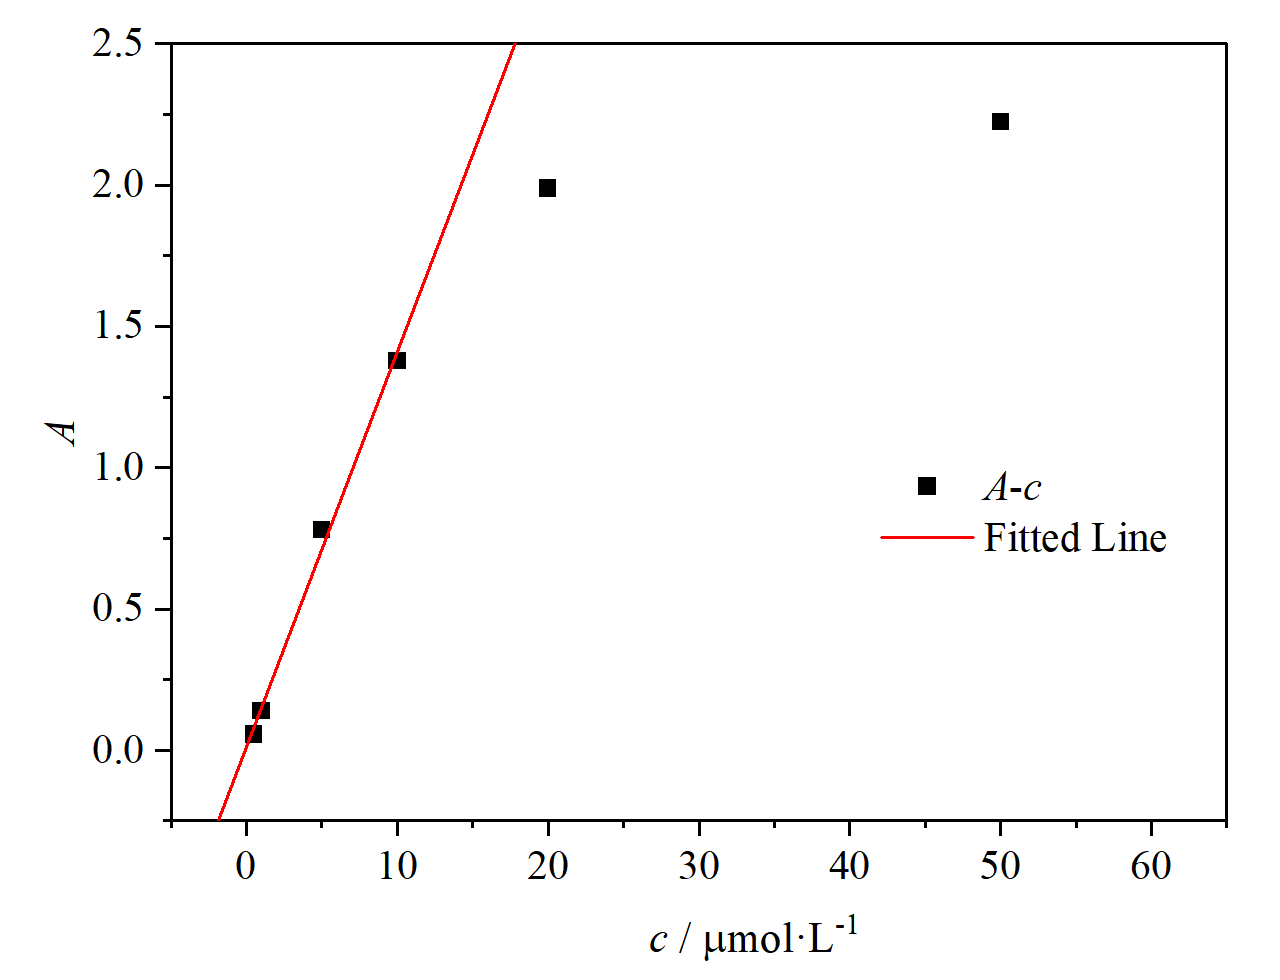
\includegraphics[width=.6\textwidth]{figures2/2-5.png}
    \bicaption{A3的吸光度-浓度关系与拟合直线}{Absorbance-Concentration Relationship and Fitting Line of A3 Molecule}
    \label{fig:7}
\end{figure}

因此,使用前四个浓度的A3乙醇溶液的吸光度-浓度进行线性拟合,得到的拟合直线如图 \ref{fig:7},拟合直线的表达式如下:

\begin{equation*}
    A = (0.140 \pm 0.007)c/\mathrm{\mu mol\cdot L^{-1}} + (0.011\pm 0.04);\quad R^2=0.9943
\end{equation*}

最终,可以求得A3的摩尔吸光系数为:
\begin{equation*}
    \varepsilon = (0.140 \pm 0.007)/1 = (0.140 \pm 0.007)\mathrm{L\cdot \mu mol^{-1}\cdot cm^{-1}}
\end{equation*}

\begin{table}[H]
    \centering
    \bicaption{A1-4的乙醇溶液的$\lambda_{\rm max}$与$\varepsilon$}{$\lambda_{\rm max}$ and $\varepsilon$ of Ethanol Solutions A1-4}
    \begin{tabular}{c|cccc}
    \toprule
     溶质 & A1 & A2 & A3 & A4 \\
     \midrule
     $\lambda_{\rm max}$/$\mathrm{nm}$  & 430.0 & 555.9 & 655.6 & 767.1\\
     $A$ & 0.533 & 0.669 & 0.779 & 0.769 \\
     $\varepsilon$/$\mathrm{L\cdot \mu mol^{-1}\cdot cm^{-1}}$ & 0.0553 & 0.134 & 0.195 & 0.256 \\
     \bottomrule
    \end{tabular}
    \label{tab:4}
\end{table}

\subsubsection{A1-4的吸收光谱}

使用可见光谱仪测量A1-4乙醇溶液的吸收光谱,如图 \ref{fig:8};对谱图进行平滑化得到图 \ref{fig:9};由图 \ref{fig:9} 可得A1-4的最大吸收光波长,如表 \ref{tab:4} 所示。

可以发现,对于类似的共轭分子A1-4,随着共轭体系的延长,分子的最大吸收波长 $\lambda_{\rm max}$ 发生显著的红移,吸收光波长变大。

\begin{figure}[H]
    \centering
    \includegraphics[width=.62\textwidth]{figures2/2-2.png}
    \bicaption{A1-4乙醇溶液的吸收光谱}{Absorption Spectrum of Ethanol Solutions of Molecules A1-4}
    \label{fig:8}
\end{figure}

\begin{figure}[H]
    \centering
    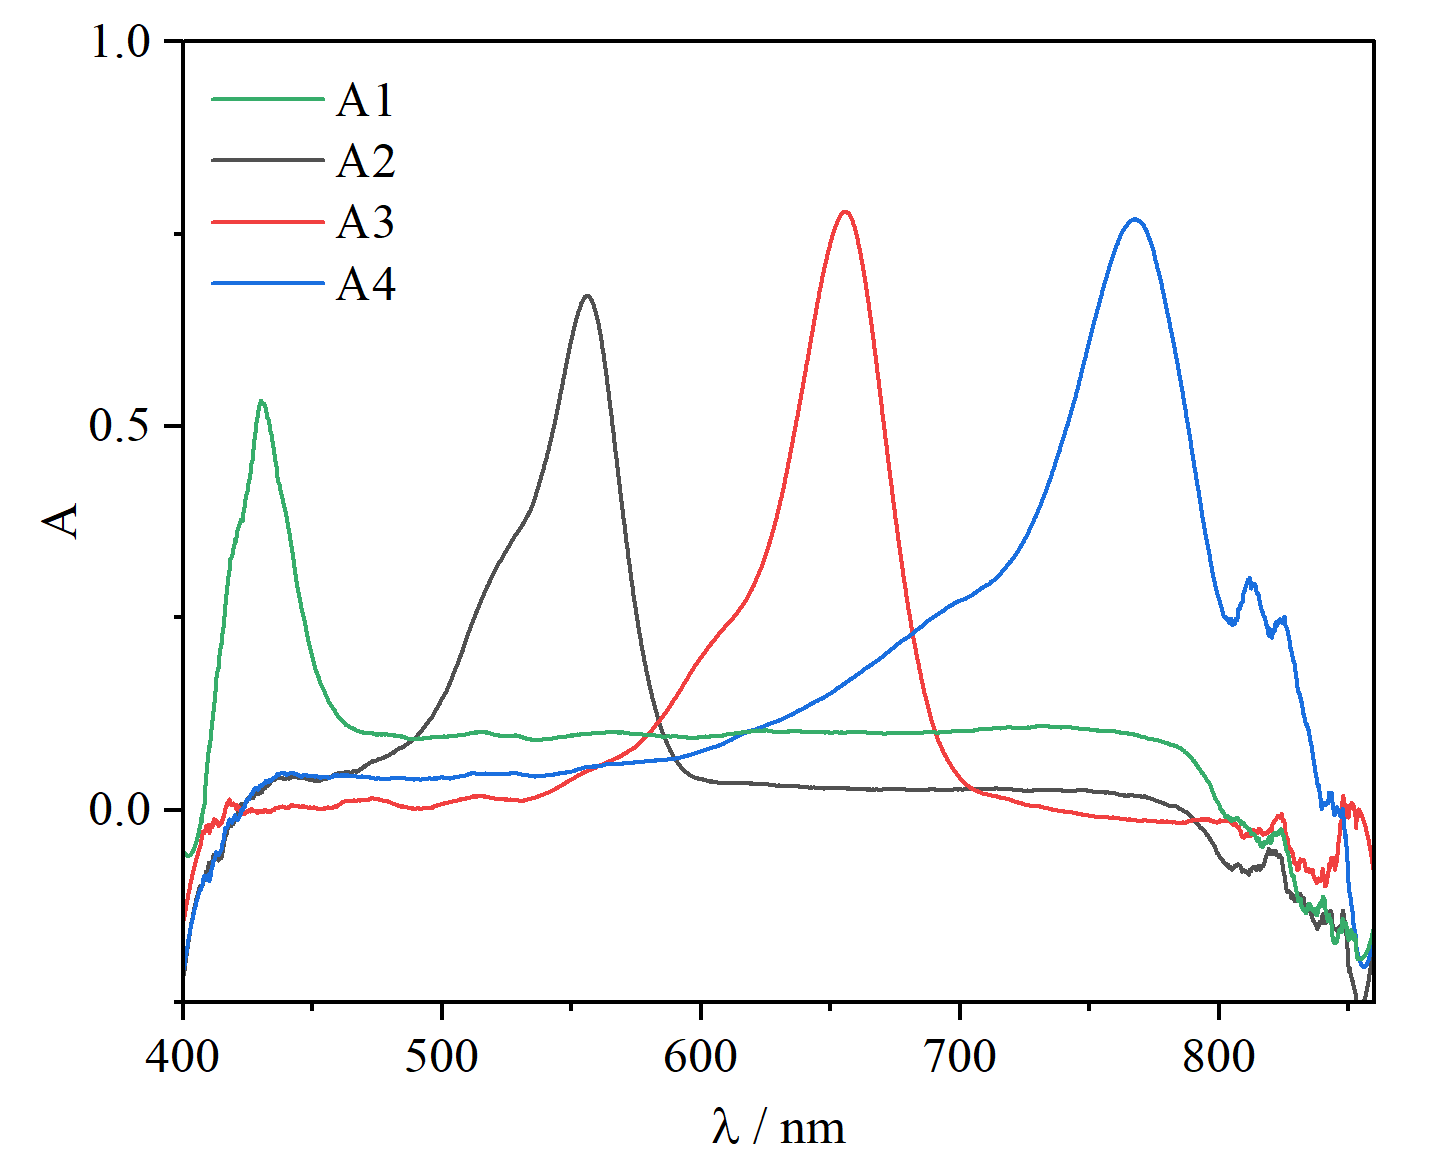
\includegraphics[width=.6\textwidth]{figures2/2-6.png}
    \bicaption{平滑化后A1-4乙醇溶液的吸收光谱}{Smoothed Absorption Spectrum of Ethanol Solutions of Molecules A1-4}
    \label{fig:9}
\end{figure}

\subsubsection{B1-2与A1的吸收光谱}

由于卤钨灯的波长范围一般为400$\thicksim$800 \si{nm}\cite{pcl2002},故为了准确测定A1、B2分子在紫外光区的吸收光谱,需要使用氘灯在紫外-可见光区测定光谱。

因此,将仪器进行调节至紫外-可见区,重新标定光谱仪,测定B1-2与A1乙醇溶液的吸收光谱,如图 \ref{fig:10};对谱图进行平滑化得到图 \ref{fig:11};由图 \ref{fig:11} 可得A1-4的最大吸收光波长,如表 \ref{tab:5} 所示。

\begin{figure}[H]
    \centering
    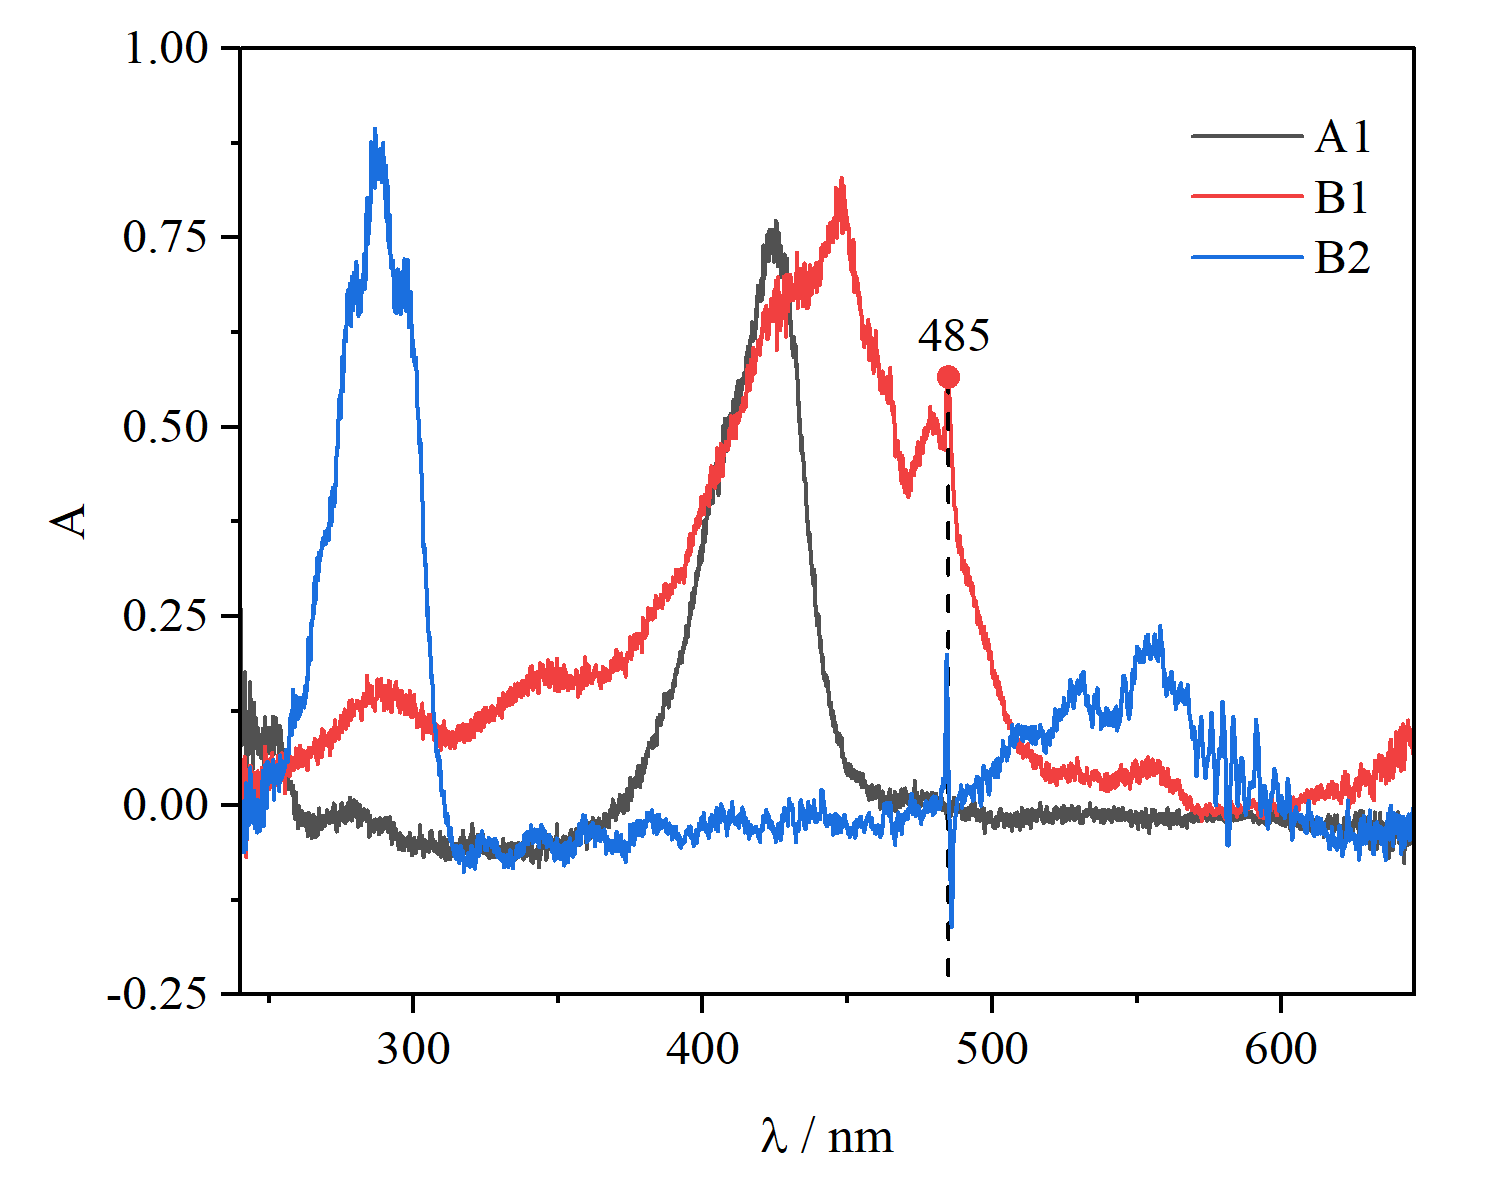
\includegraphics[width=.6\textwidth]{figures2/2-3.png}
    \bicaption{B1-2与A1乙醇溶液的吸收光谱}{Absorption Spectrum of Ethanol Solutions of Molecules B1-2 and A1}
    \label{fig:10}
\end{figure}

在图 \ref{fig:10} 中,三个分子在 $\lambda_{\rm max} = 485\mathrm{~nm}$ 处均有异常的吸收峰,这是因为如图 \ref{fig:3},它对应着氘灯的第一个发射峰的波长,在发射光强度随波长变化较大时,光强极大时可能会有额外的吸收或损耗,并不能认为这就是分子B1的特征吸收峰。

\begin{table}[H]
    \centering
    \bicaption{A1与B1-2的乙醇溶液的$\lambda_{\rm max}$与$\varepsilon$}{$\lambda_{\rm max}$ and $\varepsilon$ Wavelength of Ethanol Solutions A1, B1-2}
    \begin{tabular}{c|ccc}
    \toprule
     溶质 & B1 & B2 & A1 \\
     \midrule
     $\lambda_{\rm max}$/$\mathrm{nm}$  & 446.9 & 287.6 & 424.4 \\
     $A$ & 0.839 & 0.783 & 0.743 \\
     $\varepsilon$/$\mathrm{L\cdot \mu mol^{-1}\cdot cm^{-1}}$ & 0.0280 & 0.0783 & 0.149 \\
     \bottomrule
    \end{tabular}
    \label{tab:5}
\end{table}


\begin{figure}[H]
    \centering
    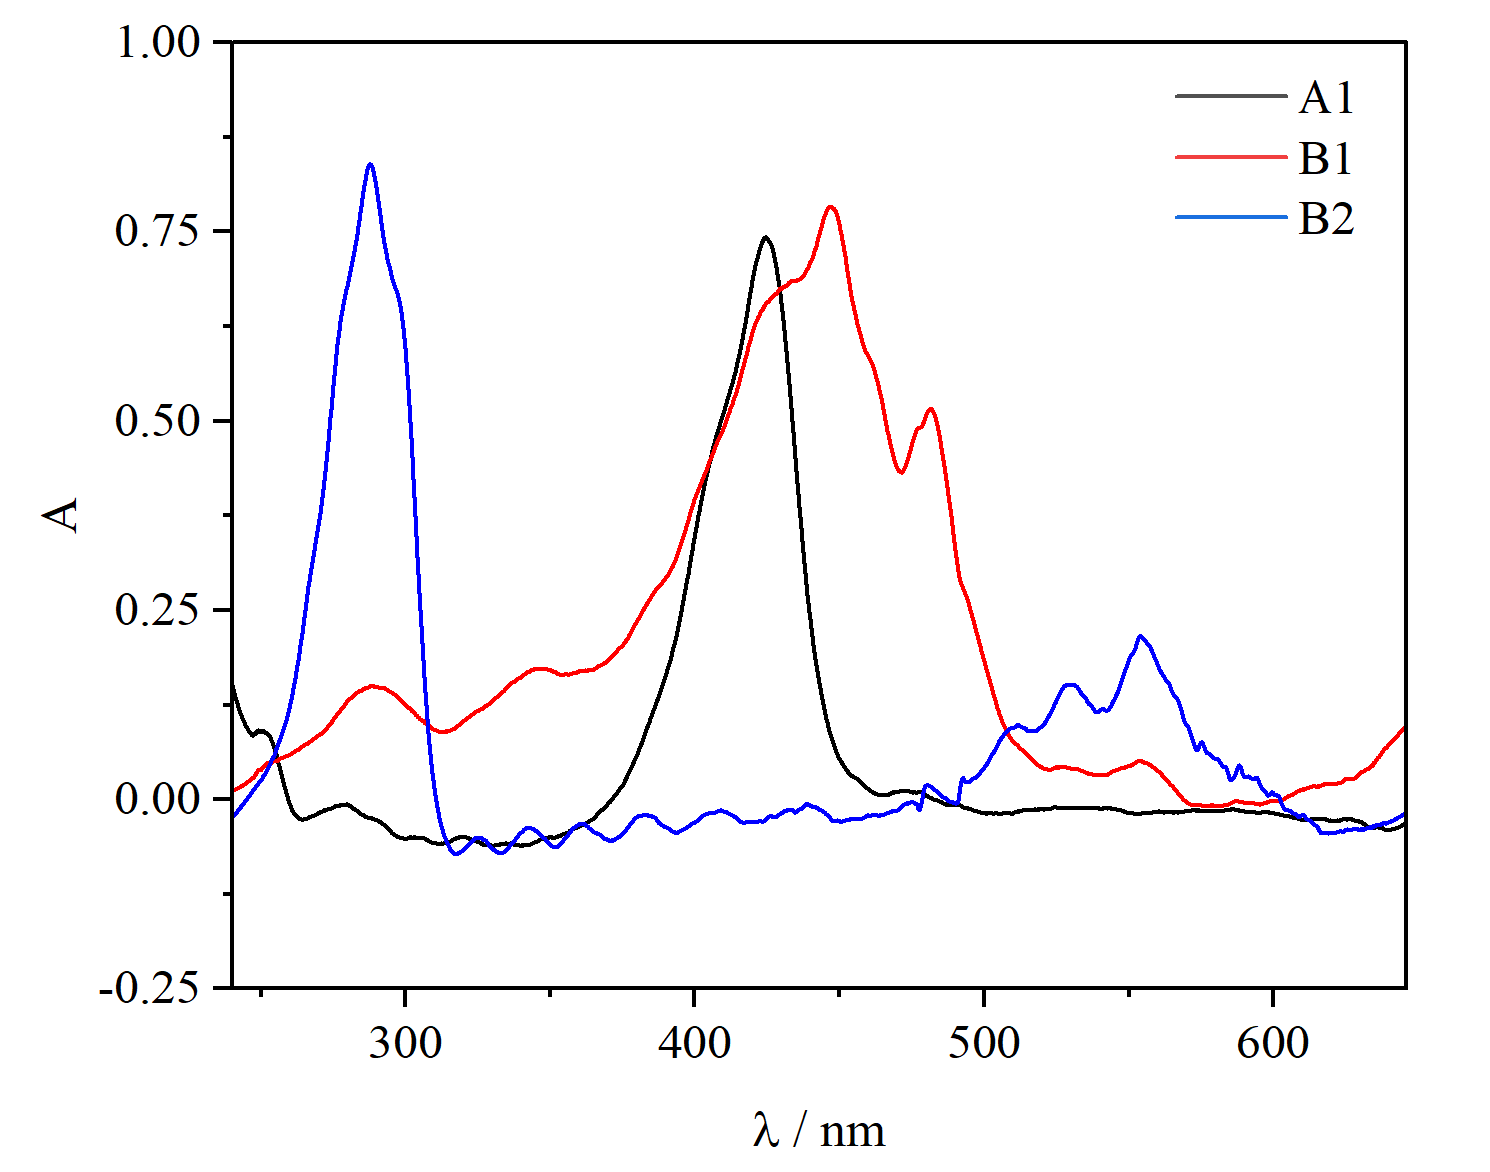
\includegraphics[width=.58\textwidth]{figures2/2-7.png}
    \bicaption{平滑化后A1-4乙醇溶液的吸收光谱}{Smoothed Absorption Spectrum of Ethanol Solutions of Molecules A1-4}
    \label{fig:11}
\end{figure}

不难发现,表 \ref{tab:5} 中使用氘灯在紫外-可见区测定的A1的最大吸收光波长比表 \ref{tab:4} 中使用卤钨灯在可见区测定的波长要小\SI{5}{nm},这是因为:根据式 \eqref{eq:1},本实验中搭建的可见光谱仪可以测定的最小光波长为\SI{400}{nm},而A1的最大吸收波长非常接近\SI{400}{nm},如图 \ref{fig:8},在光波长接近仪器测定的上下限时,由于光强减弱,信噪比提升,因此无法准确地找出A1的最大吸收峰位置,因此,使用紫外-可见光谱仪能够更准确地测定A1的最大吸光波长,故我们采纳表 \ref{tab:5} 中A1的吸光波长数据,抛弃表 \ref{tab:4} 中的对应数据。

\begin{figure}[H]
    \centering
    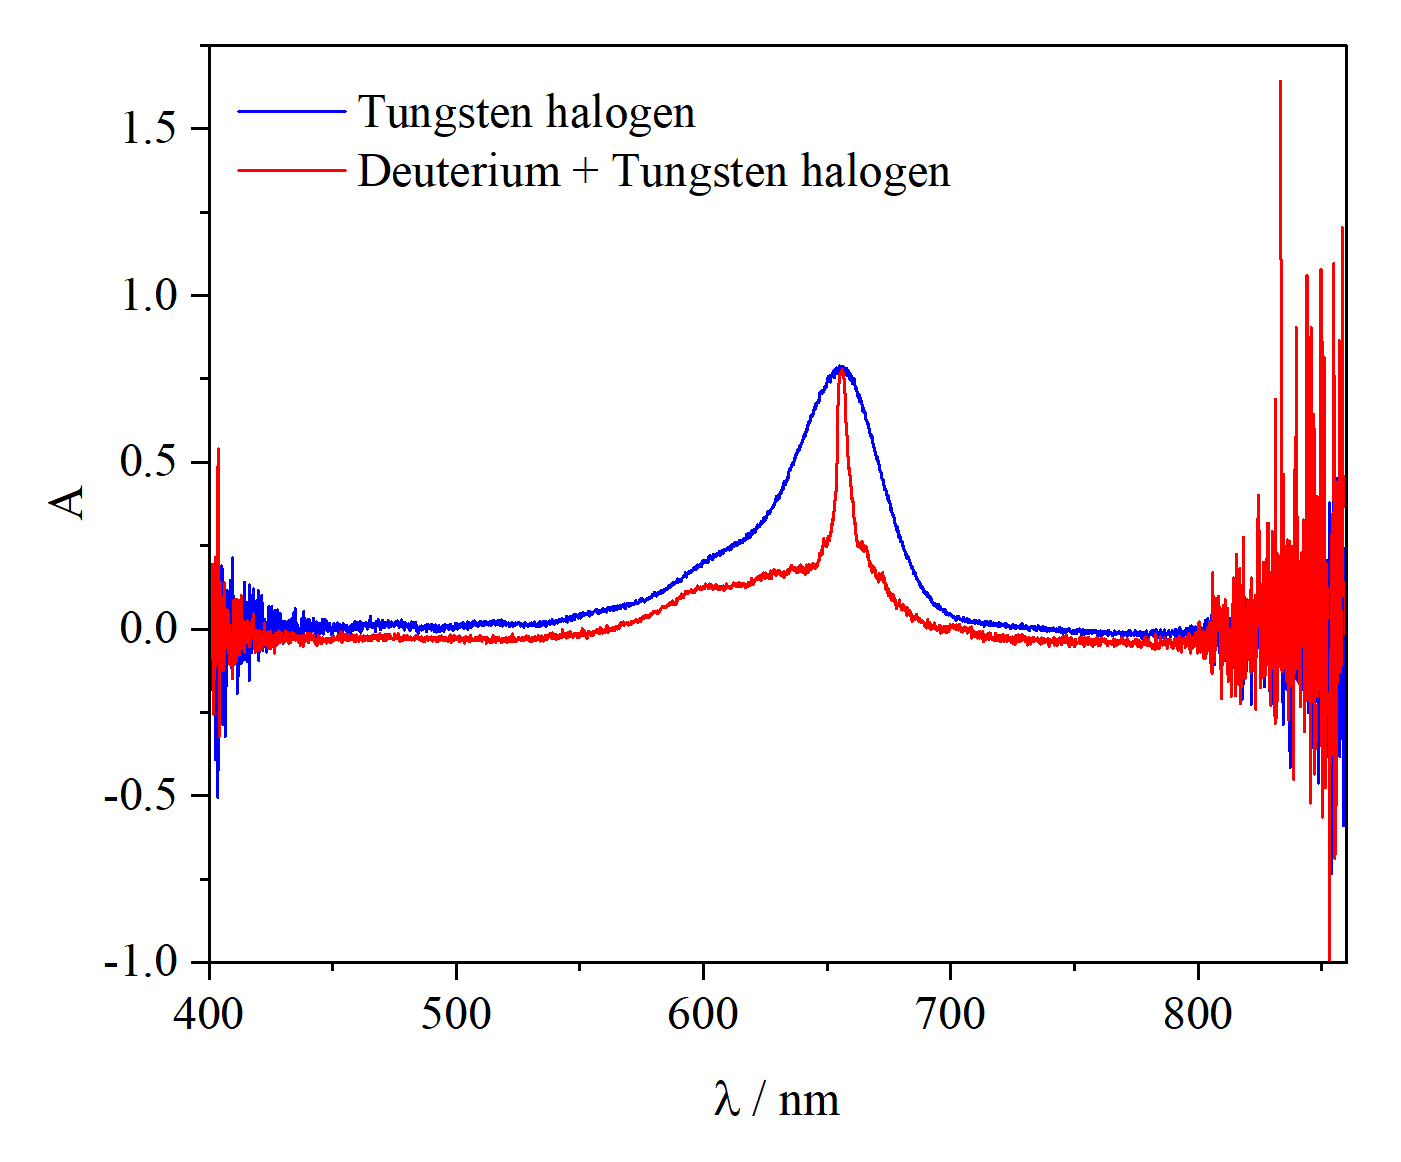
\includegraphics[width=.6\textwidth]{figures2/2-9.png}
    \bicaption{不同光源下A3乙醇溶液的吸收光谱}{Absorption Spectrum of A3 Ethanol Solution under Different Light Sources}
    \label{fig:12}
\end{figure}


\subsubsection{不同光源下A3的吸收光谱}

使用可见光谱仪测量A3乙醇溶液的吸收光谱,分别使用卤钨灯、氘灯+卤钨灯测定,得到的结果如图 \ref{fig:12}。

如图 \ref{fig:12} 可以发现,只开卤钨灯与氘灯+卤钨灯所测得的最大吸光波长与吸光率均完全一致,但是氘灯+卤钨灯能获得更窄的吸收峰,这可能是由于,如表 \ref{tab:1},氘灯在 $\lambda_{\rm max} = \SI{656}{nm}$ 处恰有一个吸收峰所导致的,而且结合图 \ref{fig:11},可以得出结论:氘灯虽然有着更强的光强、更大的波长范围,但是,其光强分布较为不均匀,存在着几个尖锐的发射峰,这会导致信噪比的不均匀,在发射光强的波长处信噪比低、在发射光弱的波长处信噪比高,为了使得得到的谱图更为规则均匀,在条件允许的前提下,有限只使用卤钨灯进行测定,例如测定A1-4的吸收光谱;而当待测物吸收光波长超出卤钨灯发射光波长范围或其他情况(光强不够透光率太低)时,则会使用氘灯进行测定;氘灯+卤钨灯的混合光源并没有使用的必要性。

\subsection{Gaussian理论计算}

本次实验中,使用Gaussian16软件进行\textit{ab. initio}的量子化学计算。

\subsubsection{分子结构的优化}

首先,在Chemdraw中画出A1-4/B1-2六个分子的结构,并使用Chem3D中mm2方法简单地初步优化分子结构;然后,使用6-31g*基组,b3lyp泛函,考虑SMD溶剂模型中的乙醇溶剂,对A1-4/B1-2六个分子进行量子化学计算,优化结构,输入文件的格式为:
\begin{code}
 \%chk=path/name.chk
 \%nproc=36
 \%mem=128GB
 # opt freq b3lyp/6-31g* scrf(smd, solvent=ethanol)
\end{code}
最终得到优化后的A1-4/B1-2六个分子结构。

\subsubsection{激发态光谱的计算}

以优化后的结构为输入,改变计算的泛函/基组,取前150个激发态,考虑SMD溶剂模型中的乙醇溶剂,进行TTDFT计算,探究不同泛函/基组计算得到最大吸收波长的不同,试图寻找最接近于实验值的泛函/基组选择,以及不同泛函/基组的计算结果与真实值的偏移规律。输入文件的格式为:
\begin{code}
 \%nproc=36
 \%mem=128GB
 # td=(nstates=150) functionals/basis_set scrf(smd, solvent=ethanol)
\end{code}

选取的泛函/基组及其对应的输入格式如表 \ref{tab:6},最终计算结果与实验值的对比如表 \ref{tab:7}。

\begin{table}[H]
    \centering
    \bicaption{选取的泛函/基组及其对应的Gaussian输入}{Selected functionals/basis sets and their Gaussian inputs}
    \begin{tabular}{ccc}
    \toprule
    编号 & 泛函/基组 & Gaussian输入 \\
    \midrule
        1 & B3LYP/6-311+G* & b3lyp/6-311+g* \\
        2 & B3LYP/6-311+G(2d,p) & b3lyp/6-311+g(2d,p) \\
        3 & B3LYP/def2-TZVP & b3lyp/def2TZVP \\
        4 & CAM-B3LYP/def2-TZVP & CAM-b3lyp/def2TZVP \\
        5 & M06-2X/def2-TZVP & M062X/def2TZVP \\
        6 & PBE0/def2-TZVP & PBE1PBE/def2TZVP \\
        \multirow{2}{*}{7} & \multirow{2}{*}{PBE38/def2-TZVP} & PBEPBE/def2-TZVP IOp(3/76=1000003750)\\
        & & IOp(3/77=0625006250) IOp(3/78=1000010000) \\
        8 & $\omega$B97XD/def2-TZVP & wB97XD/def2TZVP \\
    \bottomrule
    \end{tabular}
    \label{tab:6}
\end{table}

\begin{table}[H]
    \centering
    \bicaption{理论计算结果与实验值最大吸收波长的对比}{Comparison of Theoretical Calculation  with Experiments for Max Absorption Wavelength}
    \begin{adjustwidth}{-2cm}{-2cm}
    \begin{center}
    \begin{tabular}{cccccccccc}
    \toprule
    $\lambda_{\rm max}/\mathrm{nm}$ & 1 & 2 & 3 & 4 & 5 & 6 & 7 & 8 & 实验 \\
    \midrule
    A1 & 392.34 & 394.89 & 393.81 & 373.16 & 376.22 & 385.91 & 372.28 & 371.49 & 424.4 \\
    相对偏差 & -7.55\% & -6.95\% & -7.21\% & -12.07\% & -11.35\% & -9.07\% & -12.28\% & -12.47\% & \\
    \midrule
    A2 & 479.01 & 482.67 & 480.46 & 465.30 & 471.4 & 472.47 & 459.21 & 464.19 & 555.9 \\
    相对偏差 & -13.83\% & -13.17\% & -13.57\% & -16.30\% & -15.20\% & -15.01\% & -17.39\% & -16.50\% & \\
    \midrule
    A3 & 548.55 & 552.32 & 549.85 & 540.94 & 549.35 & 542.42 & 530.21 & 541.54 & 655.6 \\
    相对偏差 & -16.33\% & -15.75\% & -16.13\% & -17.49\% & -16.21\% & -17.26\% & -19.13\% & -17.40\% & \\
    \midrule
    A4 & 613.75 & 617.75 & 615.17 & 612.71 & 623.38 & 608.21 & 596.99 & 615.44 & 767.1 \\
    相对偏差 & -19.99\% & -19.47\% & -19.81\% & -20.13\% & -18.74\% & -20.71\% & -22.18\% & -19.77\% & \\
    \midrule
    平均偏差 & -14.43\% & -13.84\% & -14.18\% & -16.50\% & -15.37\% & -15.51\% & -17.74\% & -16.53\% & \\ 
    \toprule
    B1 & 642.61 & 645.35 & 643.92 & 538.46 & 539.05 & 622.32 & 577.47 & 525.66 & 446.9 \\
    相对偏差 & 43.79\% & 44.41\% & 44.09\% & 20.49\% & 20.62\% & 39.25\% & 29.22\% & 17.62\% & \\
    \midrule
    B2 & 294.77 & 296.29 & 294.77 & 279.3011 & 277.08 & 289.95 & 281.78 & 279.01 & 287.6 \\
    相对偏差 & 2.49\% & 3.02\% & 2.49\% & -2.89\% & -3.66\% & 0.82\% & -2.02\% & -2.99\% & \\
    \bottomrule
    \end{tabular}
    \end{center}
    \end{adjustwidth}
    \subcaption*{编号1$\thicksim$8对应着表 \ref{tab:6} 中各编号对应的计算泛函/基组}
    \label{tab:7}
\end{table}

\newpage
根据表 \ref{tab:7} 不难发现:
\begin{enumerate}
    \item 对于A1-4:
    \begin{itemize}
        \item 所有的理论计算结果均低估了最大吸收波长,即计算得到的激发态能量与实验值相比,发生了较大的蓝移,而且蓝移会随着烷基链的增加而增大;
        \item 所有结果均发生相同的偏移,说明对于A1-4而言,泛函/基组的选择并不是造成理论值与实验值偏差的主要原因,造成偏差的原因可能有
        \begin{itemize}
            \item SMD隐式溶剂模型并不适用于A1-4的乙醇溶液体系,可能存在更复杂的溶剂化作用;
            \item A1-4在乙醇溶液中的实际结构与计算得到的结构存在根本性的区别,导致理论计算基于错误的结构,自然难以得到正确结果;
            \item 随着烯烃链的增长,A1-4的分子柔性增加,各个构象转化的活化能降低,在光照下可能会改变构象,使得理论计算的输入结构与实际的吸光物种间有很大的区别,这一定程度上能够解释误差随着烯烃链增加而扩大的原因。
        \end{itemize}
        \item 对于A1-4而言,最接近实验结果的泛函/基组组合为B3LYP/6-311+G(2d,p),这可能是该泛函充分考虑了极化'(2d,p)'与非氢原子的弥散'+'所致,不过其计算误差仍然较大,B3LYP/6-311+G(2d,p)对于A1-4的计算结果优于其他组合的显著性仍有待商榷:由于计算近似的主要误差未知,无法预知充分优化误差后的计算值。因此,无法确定对于A1-4而言,何种泛函/基组组合最为适用。
    \end{itemize} 
    \item 对于B1分子:
    \begin{itemize}
        \item 与A1-4计算结果发生蓝移所截然不同的是,B1分子的计算结果均发生了大幅的红移,其原因可能与A1-4发生蓝移的原因类似:
        \begin{itemize}
            \item B1分子在乙醇溶液中的实际结构与计算结构存在区别,导致理论计算基于错误的结构;
            \item B1分子的烯烃链具有较强的柔性,在光照下会改变构象,使得计算结构与实际的吸光物种间有很大的区别。
        \end{itemize}
        \item 对于B1分子而言,最接近实际的泛函/基组组合为$\omega$B97XD/def2-TZVP,次之的是AM-B3LYP/def2-TZVP、M06-2X/def2-TZVP,而使用B3LYP泛函的组合1-3则产生了极大的偏差。
    \end{itemize}
    \item 对于B2分子:
    \begin{itemize}
        \item 由于B2分子的分子量小、不带电荷、结构刚性等,所有计算结果均取得了非常理想的结果,其中,获得最优结果的是PBE0/def2-TZVP。
    \end{itemize}
\end{enumerate}

\subsection{一维势阱模型的验证}

根据一维势阱模型,长度为 $L$ 的势阱中,量子数为 $n$ 的电子能量为
\begin{equation*}
E=\frac{n^2 h^2}{8 m_e L^2}
\end{equation*}
吸收光子从 $n$ 态跃迁到 $n + 1$ 态,光子能量等于能级差,有
\begin{equation*}
\Delta E=\frac{(2 n+1) h^2}{8 m_e L^2}=\frac{h c}{\lambda}
\end{equation*}
故预测吸收光波长
\begin{equation*}
\lambda=\frac{8 m_e c L^2}{(2 n+1) h}
\end{equation*}
最大吸收波长对应的一维势阱长度为:
\begin{equation}\label{eq:4}
L=\sqrt{\frac{(2 n+1) h \lambda_{\max }}{8 m_e c}}
\end{equation}

根据优化后的结构,使用Chemcraft软件将所有分子的键长标注在分子上,得到表 \ref{tab:9}、表 \ref{tab:8}。

\begin{table}[htbp]
    \centering
    \bicaption{B1-2分子结构优化后的键长}{Bond Lengths of B1-2 Molecules after Structural Optimization}
    \begin{tabular}{cM{15cm}}
    \toprule
    代称 & 结构 \\
    \midrule
    \textbf{B1} & 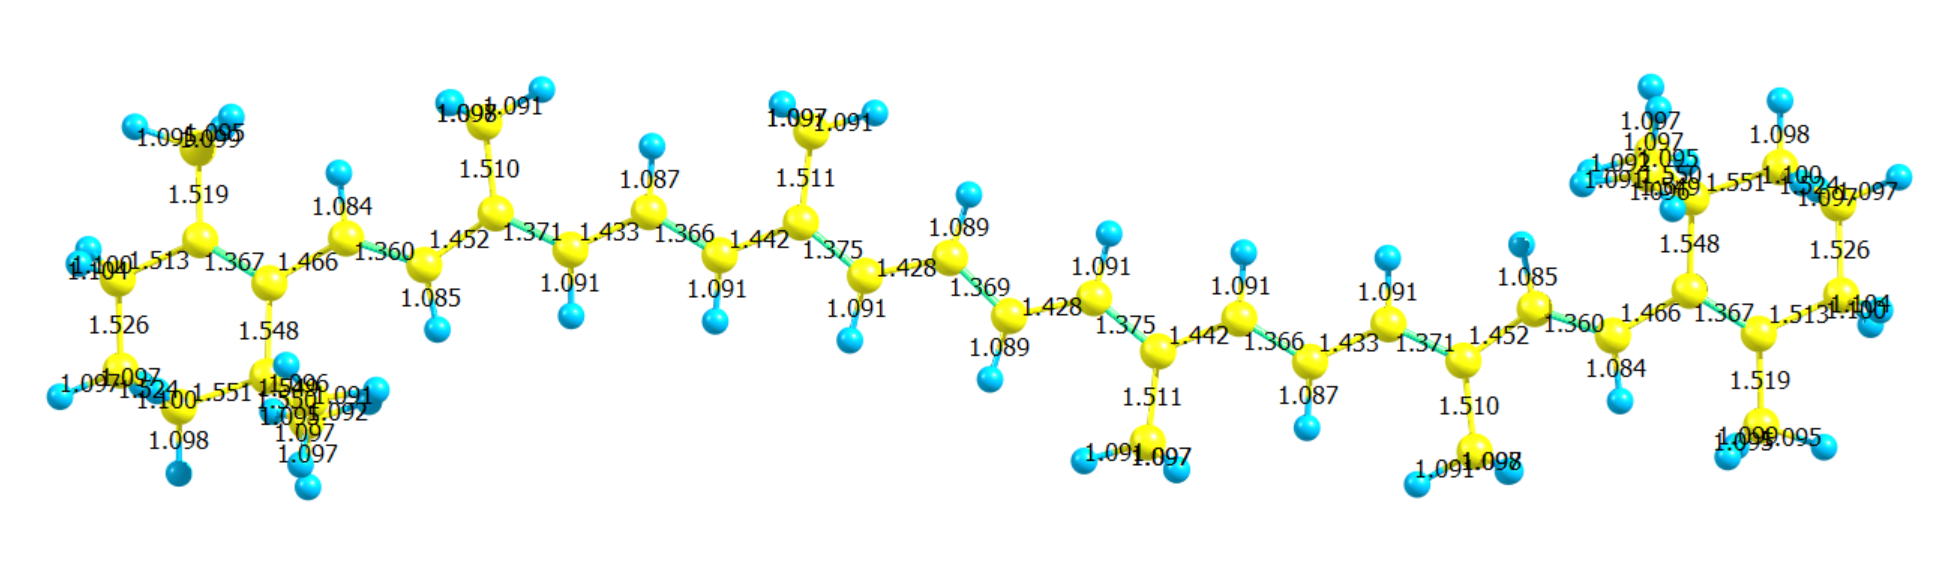
\includegraphics[scale=.45]{figures3/3-1-5.png} \\
    \textbf{B2} & 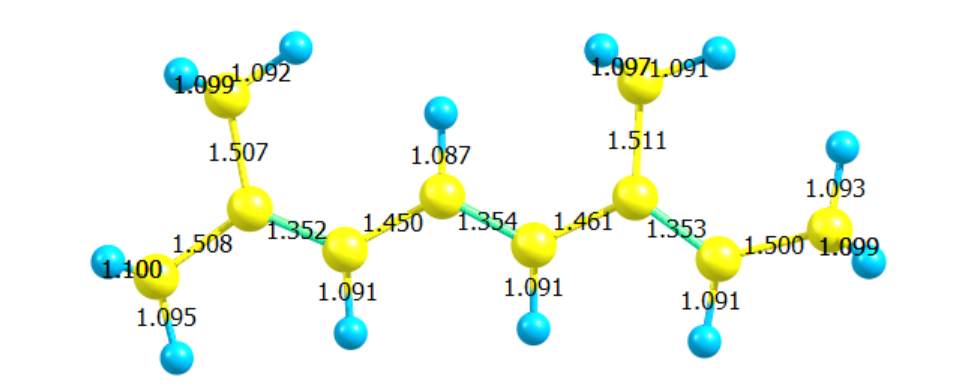
\includegraphics[scale=.4]{figures3/3-1-6.png} \\
    \bottomrule
    \end{tabular}
    \label{tab:9}
\end{table}

\begin{table}[H]
    \centering
    \bicaption{A1-4结构优化后的键长}{Bond Lengths of A1-4 Molecules after Structural Optimization}
    \begin{tabular}{cM{15cm}}
    \toprule
    代称 & 结构 \\
    \midrule
    \textbf{A1} & 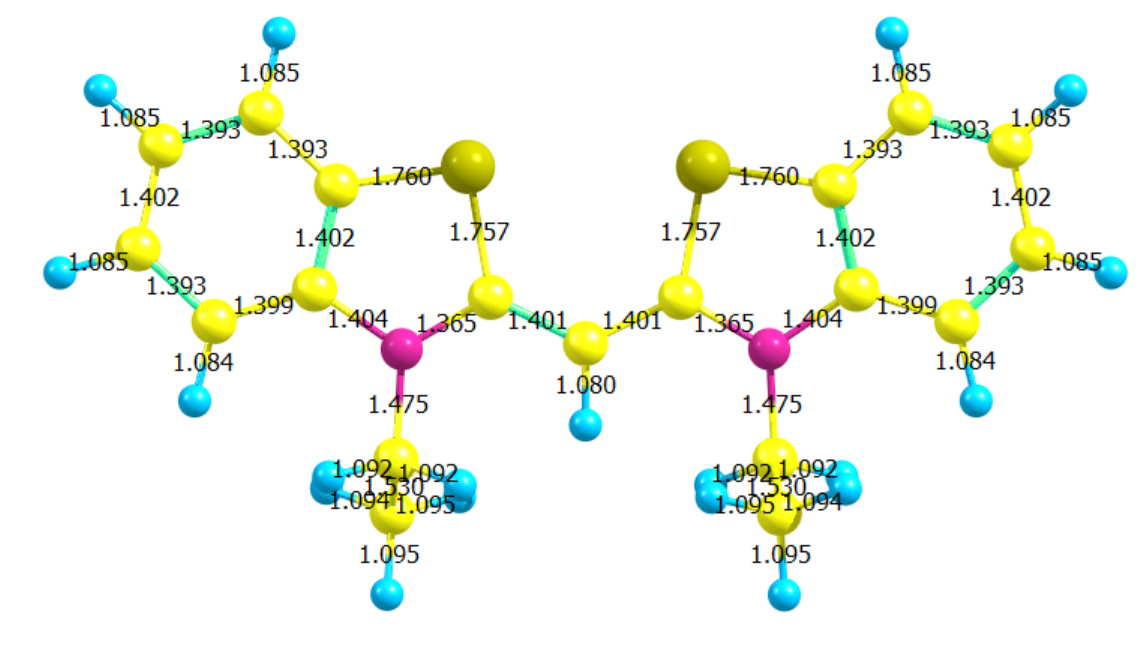
\includegraphics[scale=.43]{figures3/3-1-1.png} \\
    \textbf{A2} & 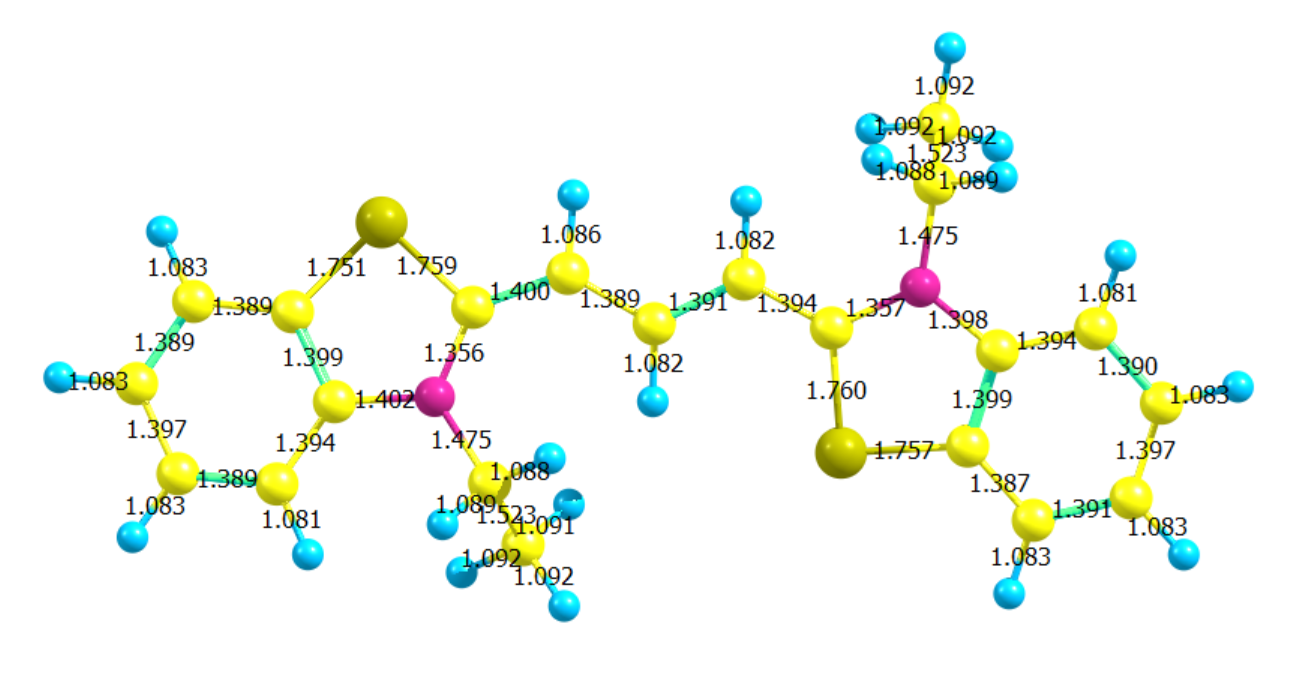
\includegraphics[scale=.43]{figures3/3-1-2.png} \\
    \textbf{A3} & 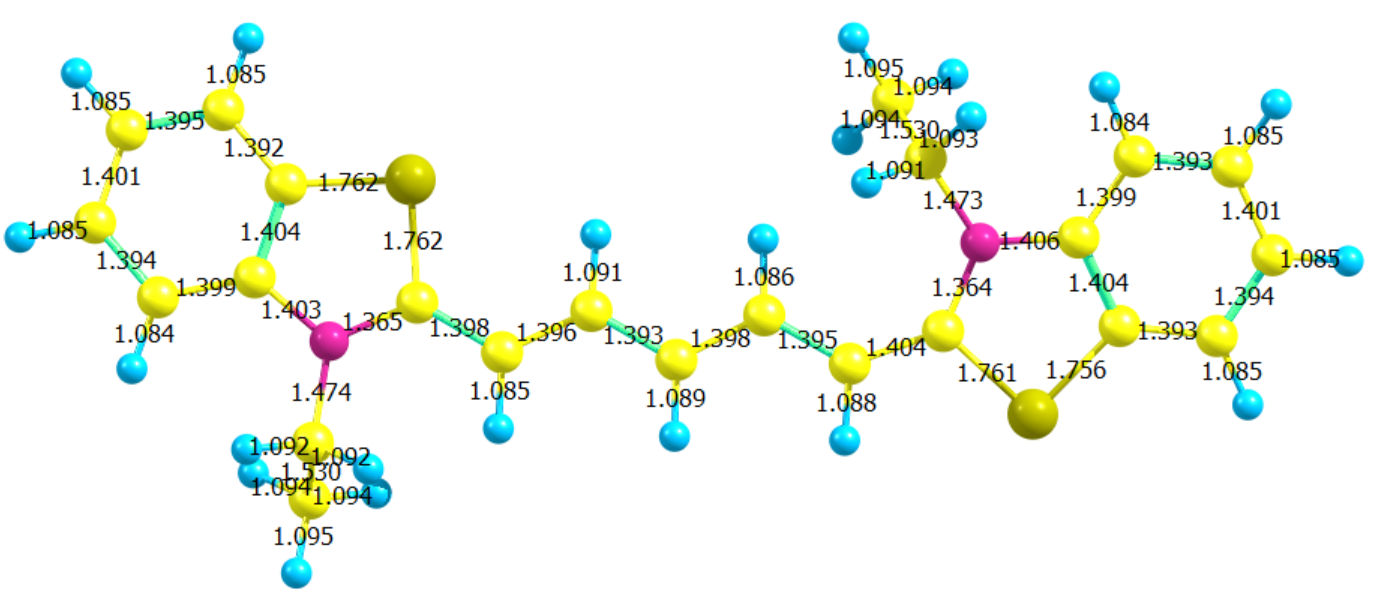
\includegraphics[scale=.43]{figures3/3-1-3.png} \\
    \textbf{A4} & 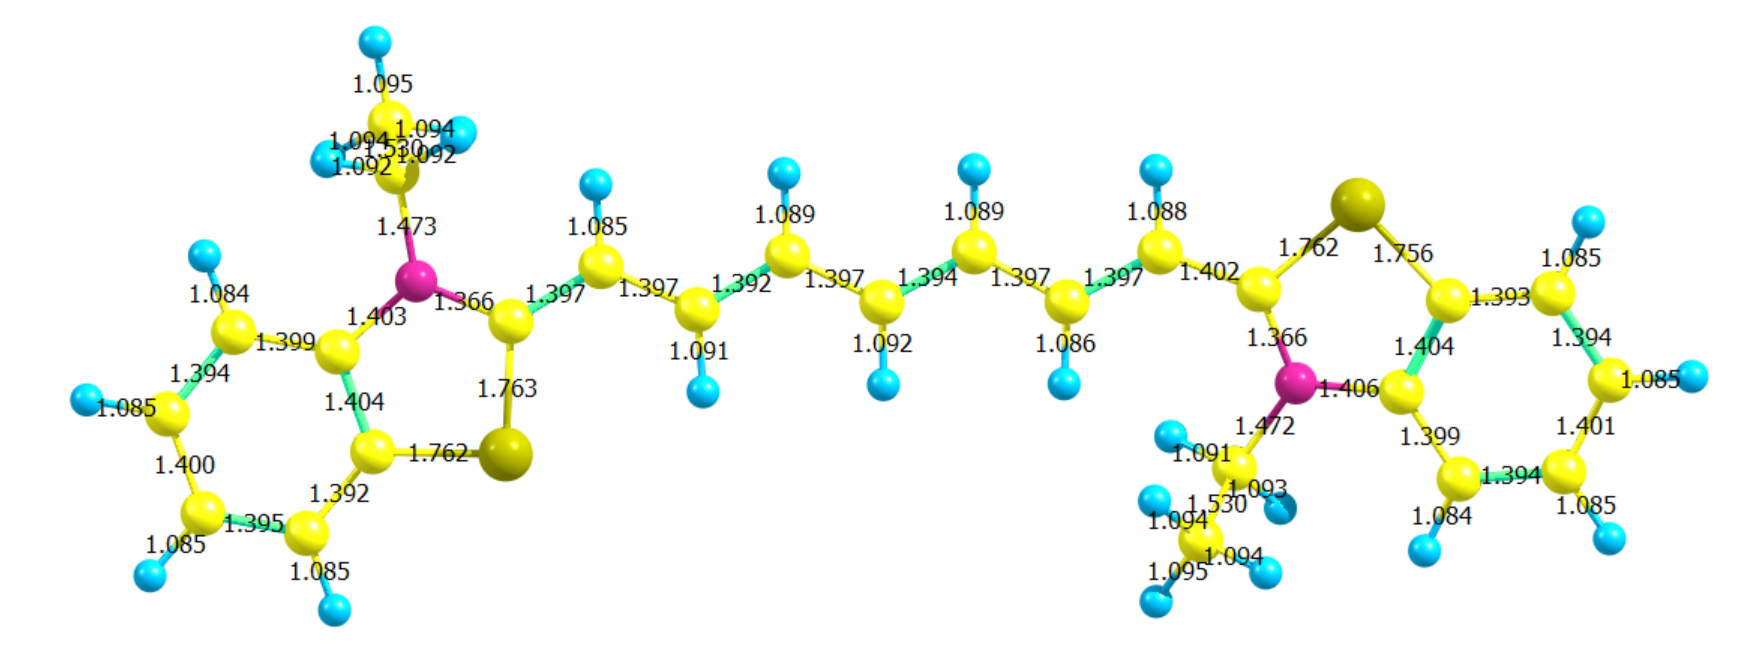
\includegraphics[scale=.43]{figures3/3-1-4.png} \\
    \bottomrule
    \end{tabular}
    \label{tab:8}
\end{table}



\subsubsection{A组分子的一维势阱模型的验证}

对于A组分子的结构通式,如图 \ref{fig:13} ,考虑多种p电子的共轭方式(双键、芳环),可以将吸收光子的基态表示为 $n=x+i$,其中 $i$ 为额外考虑的p电子的共轭对基态能级的影响,结合键长的Gaussian计算结果 \ref{tab:8},可得一维势阱的理论长度,而根据实验测定的最大吸收光波长,由式 \eqref{eq:4} 可得一维势阱的实验长度。具体地,考虑 $i$ 所对应的共轭效应,及不同 $i$ 所对应的理论和实验值的计算结果、相对偏差,得到表 \ref{tab:10}。

\begin{figure}[htbp]
    \centering
    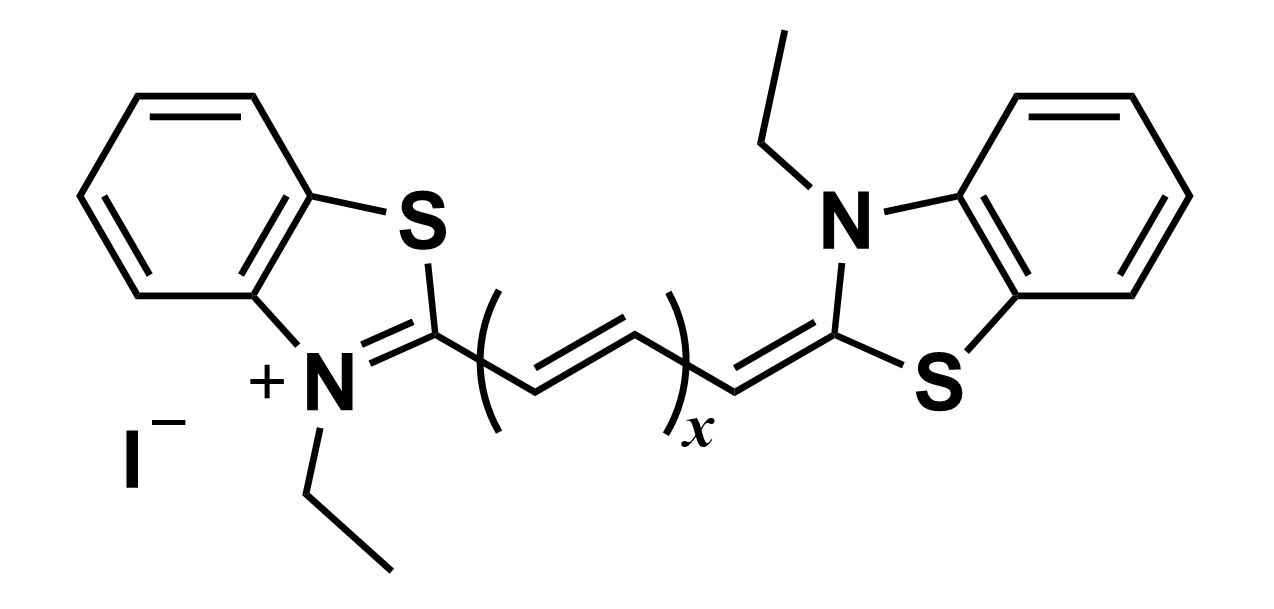
\includegraphics[width=.35\textwidth]{figures3/3-2.png}
    \bicaption{A组离子的结构通式}{General Structure of Group A Ions}
    \label{fig:13}
\end{figure}

由表 \ref{tab:10} ,根据一维势阱的长度的偏差,发现A1-4的最有可能的$i=5$,对应着共轭方式:$x+1$个C=C双键的共轭 + C-N单双键的共轭 + 2个苯环各1个双键共轭。

另外的,根据表 \ref{tab:10},还可以发现:
\begin{enumerate}
    \item $i=9/11$均产生了很大的正偏差,这是因为考虑整个苯环的共轭时,体系早已偏离一维势阱模型,需要额外地考虑二维的因素,故这样的计算结果并没有参考意义;
    \item 除去$i=9/11$的情况,在同一$i$下,A1到A4的偏差会随着双键链的长度$x$的增大而增大(绝对值减小),这可能是由于:随着$x$的增大,体系由刚性的A1转化为具有一定柔性的A4,刚性体系有利于共轭效应,而柔性体系会由于构象的熵效应,阻碍体系的共轭。也就是说,对于一维势阱长度的低估值也会逐渐减小。
\end{enumerate}

\newpage
\begin{table}[htbp]
    \centering
    \bicaption{A组离子一维势阱模型的验证}{Validation of the One-Dimensional Potential Well Model for Group A Ions}
    \begin{tabular}{cc|ccccc}
        \toprule
        \multirow{2}{*}{$i$} & \multirow{2}{*}{考虑的共轭效应} & \multicolumn{5}{c}{一维势阱的长度(\si{\r{A}})与相对偏差}\\
        & & 编号 & A1 & A2 & A3 & A4 \\
        \midrule
        \multirow{3}{*}{\textbf{1}} & \multirow{3}{*}{$x+1$个C=C双键的共轭} & 理论 & 1.401 & 4.174 & 6.980 & 9.771 \\
        & & 实验 & 6.214 & 9.181 & 11.798 & 14.470 \\
        & & 偏差 & -77.45\% & -54.54\% & -40.84\% & -32.48\%\\
        \midrule
        \multirow{3}{*}{\textbf{2}} & \multirow{3}{*}{\textbf{1} + C=N双键的共轭} & 理论 & 4.167 & 6.930 & 9.748 & 12.539 \\
        & & 实验 & 8.022 & 10.864 & 13.377 & 15.997 \\
        & & 偏差 & -48.06\% & -36.21\% & -27.13\% & -21.62\%\\
        \midrule
        \multirow{3}{*}{\textbf{3}} & \multirow{3}{*}{\textbf{2} + C-N单键的共轭} & 理论 & 5.532 & 8.286 & 11.113 & 13.905 \\
        & & 实验 & 9.492 & 12.318 & 14.789 & 17.391 \\
        & & 偏差 & -41.72\% & -32.73\% & -24.86\% & -20.05\%\\
        \midrule
        \multirow{3}{*}{\textbf{5}} & \multirow{3}{*}{\textbf{3} + 2个苯环各1个双键共轭} & 理论 & 11.144 & 13.884 & 16.730 & 19.675 \\
        & & 实验 & 11.899 & 14.805 & 17.270 & 19.887 \\
        & & 偏差 & -6.35\% & -6.22\% & -3.13\% & -1.07\%\\
        \midrule
        \multirow{3}{*}{\textbf{9}} & \multirow{3}{*}{\textbf{3} + 2个苯环共轭} & 理论 & 22.296 & 25.002 & 27.882 & 30.673 \\
        & & 实验 & 15.638 & 18.816 & 21.385 & 24.117 \\
        & & 偏差 & 42.57\% & 32.87\% & 30.38\% & 27.18\%\\
        \midrule
        \multirow{3}{*}{\textbf{11}} & \multirow{3}{*}{\textbf{9} + 2个硫原子共轭} & 理论 & 25.816 & 28.472 & 31.400 & 34.191 \\
        & & 实验 & 17.206 & 20.530 & 23.170 & 25.975 \\
        & & 偏差 & 50.04\% & 38.68\% & 35.52\% & 31.63\%\\
        \bottomrule
    \end{tabular}
    \label{tab:10}
    \subcaption*{“考虑的共轭效应”一栏中,加粗的数字为已经考虑的共轭效应所对应的 $i$ 值}
    \subcaption*{第三过渡周期的硫原子的半径较大,难以与第二过渡周期的碳、氮共轭,故最后考虑}
\end{table}

\subsubsection{B组分子的一维势阱模型的验证}

由表 \ref{tab:0} 中B组分子的结构,与A组离子不同的是,B组分子的共轭体系相对固定,B1的$n=11$、B2的$n=3$。根据表 \ref{tab:8} 中使用Gaussian计算得到的结构计算一维势阱的实际长度,根据实验结果与式 \eqref{eq:4} 可得理论长度,如表 \ref{tab:11}。

\begin{table}[H]
    \centering
    \bicaption{B组分子一维势阱模型的验证}{Validation of the One-Dimensional Potential Well Model for Group B Molecules}
    \begin{tabular}{ccccc}
    \toprule
        编号 & n & 实际波长/\si{nm} & 理论波长/\si{nm} & 相对偏差\\
        \midrule
        B1 & 11 & 29.489 & 17.656 & 55.69\% \\
        B2 & 3 & 6.97 & 7.814 & 12.11\% \\
        \bottomrule
    \end{tabular}
    \label{tab:11}
\end{table}

由表 \ref{tab:11} 可以发现,B2分子理论与实际的偏差尚且在可接受的范围内,而B1分子理论与实际的偏差极大,为此,不妨怀疑:是否是B1分子的HOMO和LUMO中并未完全共轭?为此,使用GaussianView 6软件画出B1分子的前线轨道,如图 \ref{fig:14}。

\begin{figure}
    \centering
    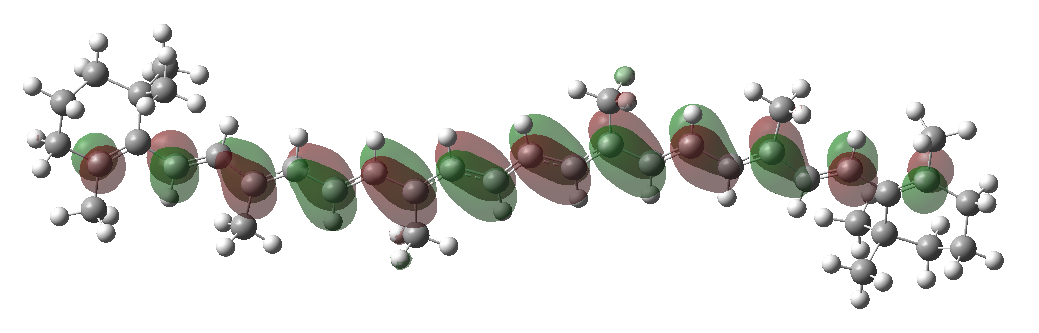
\includegraphics[width=0.7\textwidth]{figures3/3-3-1.png}
    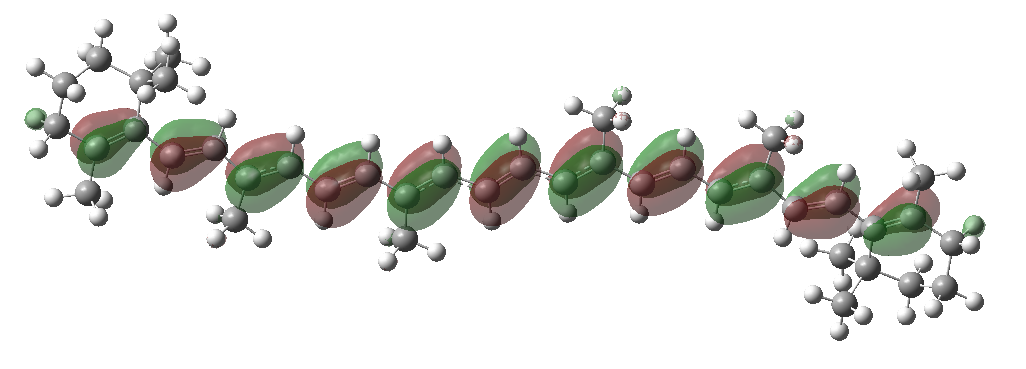
\includegraphics[width=0.7\textwidth]{figures3/3-3-2.png}
    \bicaption{B1分子的HOMO和LUMO轨道}{HOMO ans LUMO Orbital of Molecule B1}
    \label{fig:14}
\end{figure}

由图 \ref{fig:14} 可以发现,B1的前线轨道中,所有双键均参与了共轭。所以,造成B1分子不符合一维势箱模型的主要原因应当为:B1分子柔性大,在光照条件下会发生构象的转变,从而使得体系大大偏离一维势箱模型。


















